
\documentclass[11pt]{article}\usepackage[]{graphicx}\usepackage[]{color}
%% maxwidth is the original width if it is less than linewidth
%% otherwise use linewidth (to make sure the graphics do not exceed the margin)
\makeatletter
\def\maxwidth{ %
  \ifdim\Gin@nat@width>\linewidth
    \linewidth
  \else
    \Gin@nat@width
  \fi
}
\makeatother

\definecolor{fgcolor}{rgb}{0.345, 0.345, 0.345}
\newcommand{\hlnum}[1]{\textcolor[rgb]{0.686,0.059,0.569}{#1}}%
\newcommand{\hlstr}[1]{\textcolor[rgb]{0.192,0.494,0.8}{#1}}%
\newcommand{\hlcom}[1]{\textcolor[rgb]{0.678,0.584,0.686}{\textit{#1}}}%
\newcommand{\hlopt}[1]{\textcolor[rgb]{0,0,0}{#1}}%
\newcommand{\hlstd}[1]{\textcolor[rgb]{0.345,0.345,0.345}{#1}}%
\newcommand{\hlkwa}[1]{\textcolor[rgb]{0.161,0.373,0.58}{\textbf{#1}}}%
\newcommand{\hlkwb}[1]{\textcolor[rgb]{0.69,0.353,0.396}{#1}}%
\newcommand{\hlkwc}[1]{\textcolor[rgb]{0.333,0.667,0.333}{#1}}%
\newcommand{\hlkwd}[1]{\textcolor[rgb]{0.737,0.353,0.396}{\textbf{#1}}}%

\usepackage{framed}
\makeatletter
\newenvironment{kframe}{%
 \def\at@end@of@kframe{}%
 \ifinner\ifhmode%
  \def\at@end@of@kframe{\end{minipage}}%
  \begin{minipage}{\columnwidth}%
 \fi\fi%
 \def\FrameCommand##1{\hskip\@totalleftmargin \hskip-\fboxsep
 \colorbox{shadecolor}{##1}\hskip-\fboxsep
     % There is no \\@totalrightmargin, so:
     \hskip-\linewidth \hskip-\@totalleftmargin \hskip\columnwidth}%
 \MakeFramed {\advance\hsize-\width
   \@totalleftmargin\z@ \linewidth\hsize
   \@setminipage}}%
 {\par\unskip\endMakeFramed%
 \at@end@of@kframe}
\makeatother

\definecolor{shadecolor}{rgb}{.97, .97, .97}
\definecolor{messagecolor}{rgb}{0, 0, 0}
\definecolor{warningcolor}{rgb}{1, 0, 1}
\definecolor{errorcolor}{rgb}{1, 0, 0}
\newenvironment{knitrout}{}{} % an empty environment to be redefined in TeX

\usepackage{alltt}

% margins, size, formatting

\oddsidemargin=0in
\evensidemargin=0in
\topmargin=0in
\textwidth=6.5in
\textheight=9.5in
\parindent = 0 in
%\pagestyle{plain}
\pagestyle{plain}

\usepackage{amsmath,amssymb,amsthm, amsfonts}
\usepackage{array}
\usepackage{fancyhdr}
%\pagestyle{plain}
\pagestyle{fancy}
\usepackage[bottom=0.5in]{geometry}
%\usepackage{listings}
%\usepackage{inconsolata}

\lhead{\textbf{Group 3: Data Analysis\\ Spring 2014}}
\rhead{\textbf{Nick Cummings, Liza Nicoll \\ Emily Ramos and Yiding Zhang}}
\cfoot{}
\IfFileExists{upquote.sty}{\usepackage{upquote}}{}

\begin{document}

\section{Group Analysis} 

%------------------------------------------------

\subsection{Introduction}






%------------------------------------------------

\subsection{Summary of the Dataset}

%------------------------------------------------

\textbf{Weight}\\
   
Weight was measured for 507 physically active individuals - 247 men and 260 women. The distribution ranged from 42 kilograms to 116.4 kilograms. The mean weight and quartiles was signifigantly higher for men than women. We observe several outliers in the upper end of the range for both men and women. This may be due to the fact that the population sampled included a number of highly physicaly fit individuals with higher than average muscle mass.

\begin{knitrout}
\definecolor{shadecolor}{rgb}{0.969, 0.969, 0.969}\color{fgcolor}
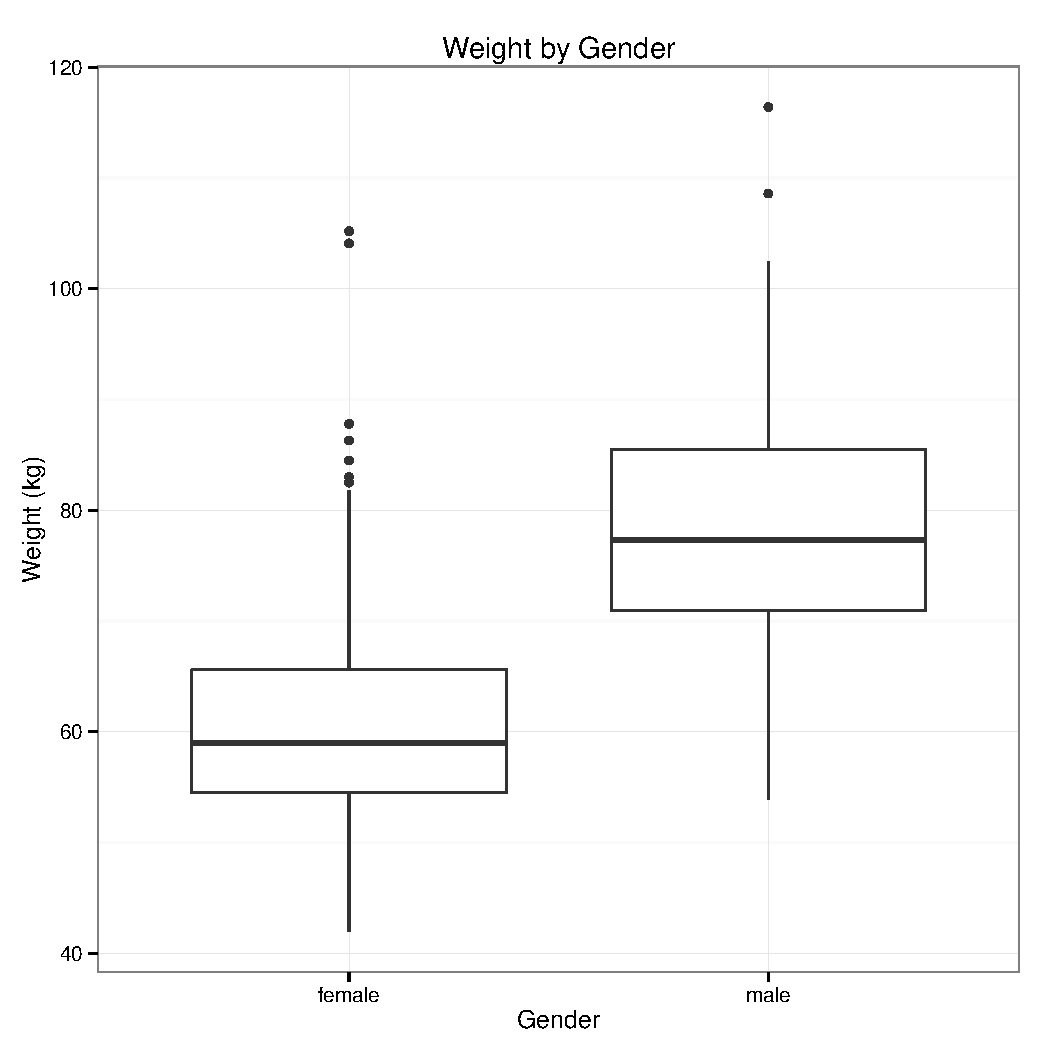
\includegraphics[width=\maxwidth]{figure/weight_plot} 

\end{knitrout}


%------------------------------------------------

\textbf{Bitrochanteric Diameter and Hip Girth}\\
 
Bitrochanteric diameter is the distance between the outer points of the hips and hip girth is the circumference of the hip area measured at the level of the bitrochanteric diameter. The density distributions for both measures are normally distributed (though hip girth is skewed slightly right) and very similar in distribution for both men and women. A scatter plot of hip girth vs. weight suggests that weight increases linerally with increase in hip girth.

\begin{knitrout}
\definecolor{shadecolor}{rgb}{0.969, 0.969, 0.969}\color{fgcolor}
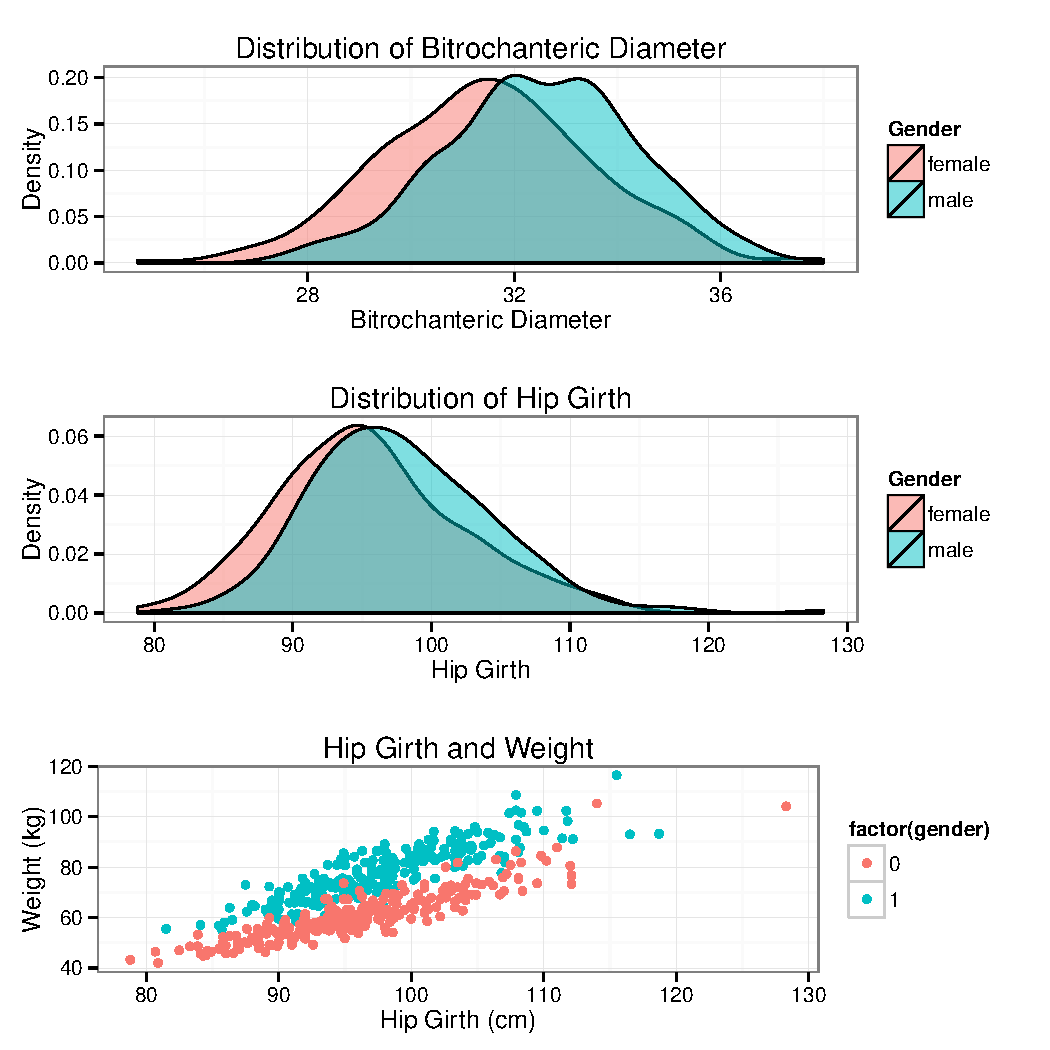
\includegraphics[width=\maxwidth]{figure/hip_plots} 

\end{knitrout}



\begin{knitrout}
\definecolor{shadecolor}{rgb}{0.969, 0.969, 0.969}\color{fgcolor}
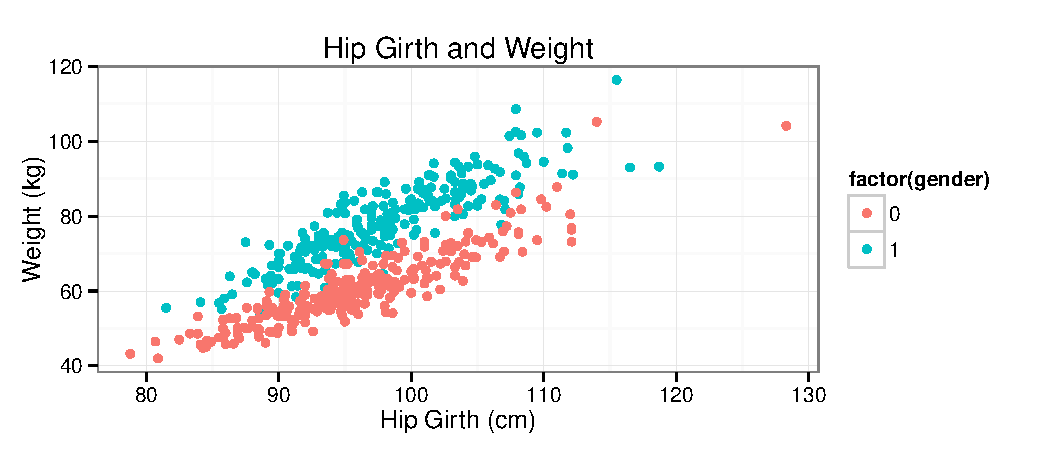
\includegraphics[width=\maxwidth]{figure/hipgirth_plot} 

\end{knitrout}


%------------------------------------------------

\textbf{Chest and Shoulder}\\
   
Chest girth was measured at the nipple line in males and just above breast tissue in females at mid-expiration and shoulder girth was measured over deltoid muscles in both males and females. The density distributions for the two variables are quite similar. Women have narrower, though slightly skeewed, distribution with a much lower mean than that of the men. The scatterplots are also similar in that the regression lines for men and women are nearly identical, indicating that weight increases linearly with increase in shoulder girth, independant of gender.

\begin{knitrout}
\definecolor{shadecolor}{rgb}{0.969, 0.969, 0.969}\color{fgcolor}
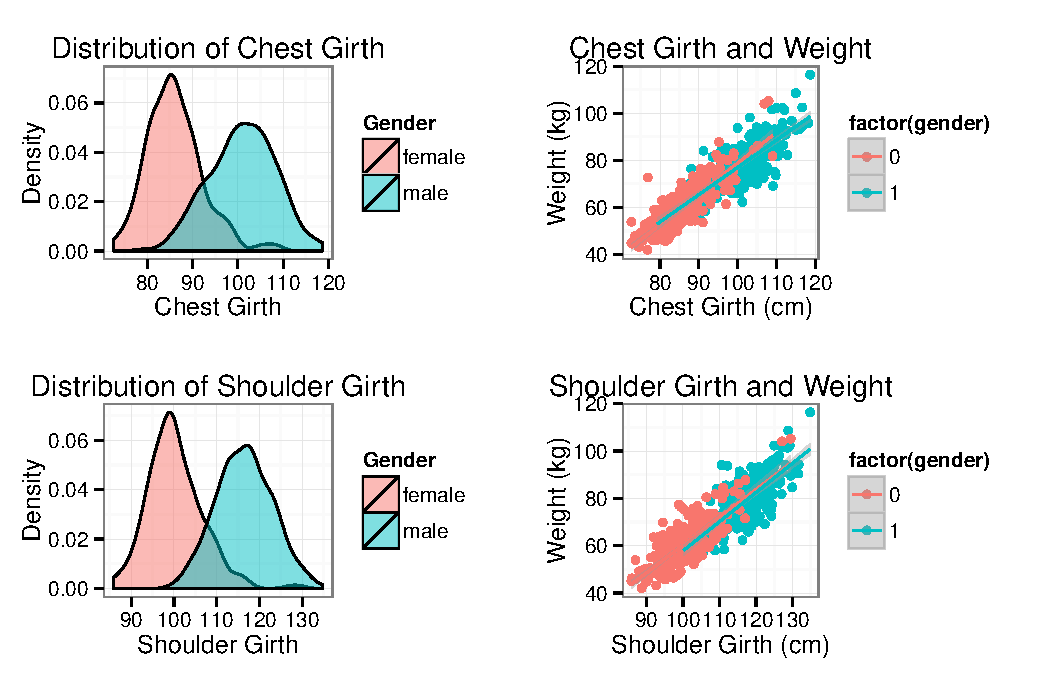
\includegraphics[width=\maxwidth]{figure/chest_plots} 

\end{knitrout}


%------------------------------------------------

\textbf{Wrist and Navel}\\
   
Wrist minimum girth is an average of right and left girths and navel (or abdominal) girth was measured at umbilicus and the iliac crest, using the iliac crest as a landmark. Wrist girth is bimodally distributed, but when divided into male and female, the distributions are normal with some outliers at the high end of the range for females. The distributions for navel girth is normal and remarkably similar for males and females. The scatterplot of navel girth against weight shows a linear relationship with weight increasing with increased naval girth.

\begin{knitrout}
\definecolor{shadecolor}{rgb}{0.969, 0.969, 0.969}\color{fgcolor}
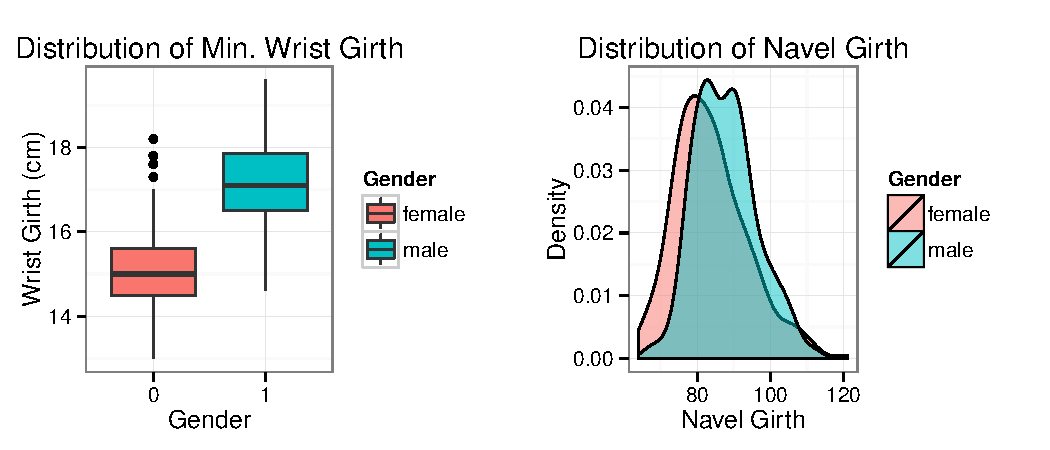
\includegraphics[width=\maxwidth]{figure/navel_plots} 

\end{knitrout}


\begin{knitrout}
\definecolor{shadecolor}{rgb}{0.969, 0.969, 0.969}\color{fgcolor}
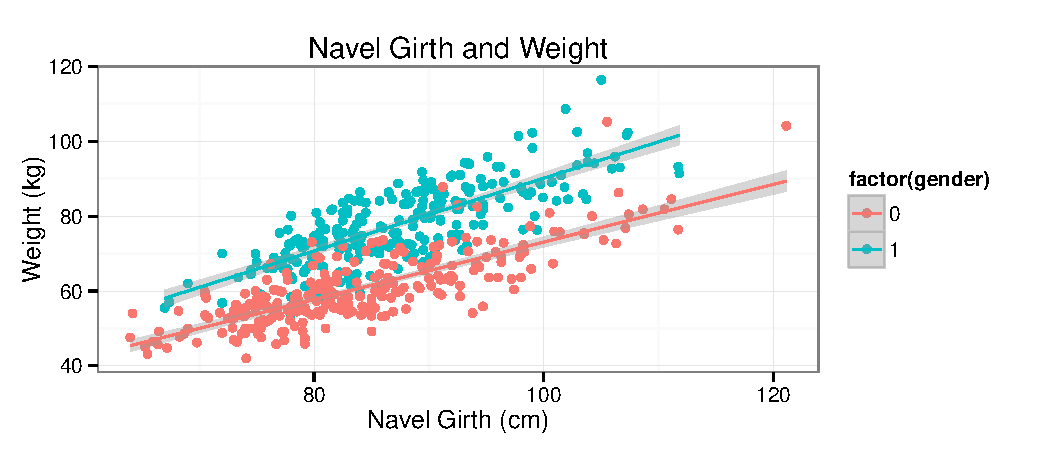
\includegraphics[width=\maxwidth]{figure/navelgirth_plot} 

\end{knitrout}


%------------------------------------------------

\subsection{Initial Multiple Linear Regression Model}

%------------------------------------------------

The initial model we are interested in fitting is of the form:\\

weight$_i = \beta_0 + \beta_1$ shoulder$_{i} + \beta_2$ chest$_{i} + \beta_3$ waist$_{i} + \beta_4$ navel$_{i}$ + \beta_5$ hip$_{i} + \beta_6$ thigh$_{i} + \beta_7$ bicep$_{i} + \beta_8$ forearm$_{i} + \beta_9$ knee$_{i} + \beta_{10}$ calf$_{i} + \beta_{11}$ ankle.min$_{i} + \beta_{12}$ wrist.min$_{i} + \beta_{13}$ height$_{i}$ \\

Text describing why this model, Where we got the model\\

\begin{knitrout}
\definecolor{shadecolor}{rgb}{0.969, 0.969, 0.969}\color{fgcolor}\begin{kframe}
\begin{alltt}
\hlstd{mlr1} \hlkwb{<-} \hlkwd{lm}\hlstd{(weight} \hlopt{~} \hlstd{shoulder} \hlopt{+} \hlstd{chest} \hlopt{+} \hlstd{waist} \hlopt{+} \hlstd{navel} \hlopt{+} \hlstd{hip} \hlopt{+} \hlstd{thigh} \hlopt{+} \hlstd{bicep} \hlopt{+}
    \hlstd{forearm} \hlopt{+} \hlstd{knee} \hlopt{+} \hlstd{calf} \hlopt{+} \hlstd{ankle.min} \hlopt{+} \hlstd{wrist.min} \hlopt{+} \hlstd{height,} \hlkwc{data} \hlstd{= body)}
\hlstd{mlr1}
\end{alltt}
\begin{verbatim}
## 
## Call:
## lm(formula = weight ~ shoulder + chest + waist + navel + hip + 
##     thigh + bicep + forearm + knee + calf + ankle.min + wrist.min + 
##     height, data = body)
## 
## Coefficients:
## (Intercept)     shoulder        chest        waist        navel  
##   -1.20e+02     7.81e-02     1.98e-01     3.40e-01     1.17e-03  
##         hip        thigh        bicep      forearm         knee  
##    2.40e-01     3.14e-01     5.47e-02     5.32e-01     3.01e-01  
##        calf    ankle.min    wrist.min       height  
##    4.04e-01    -9.63e-03    -1.18e-01     3.28e-01
\end{verbatim}
\end{kframe}
\end{knitrout}


Interpret the model\\

Discuss potential uses for models of this data (finding ideal weight based on skeletal measurements?) and potential problems for applying to whole population (all participants were physically fit)

%------------------------------------------------

\section{Individual Analysis}

%------------------------------------------------

\subsection{Regression Trees}

%------------------------------------------------

\subsection{Resampling Inference or something}

%------------------------------------------------

\subsection{Not sure what Yiding decided on}

%------------------------------------------------

\subsection{Model Selection}


\end{document}
